

\documentclass[../../main.tex]{subfiles}



\begin{document}
\section{Introducción}
En el presente informe se desarrollra el análisis te\'orico de un amplificador implementado a partir de transistores, la construcción de dicho amplificador y la medición de sus características. El objetivo de este an\'alisis es comprobar en la pr\'actica algunos de los aspectos mas destacados de los circuitos estudiados durante el curso de Electr\'onica I, dentro de un marco de simulación de recursos escasos.

\section{Amplificador}
Se construyó el amplificador de la figura \ref{fig:cir}. Tal como se observa en ella, el circuito es un colector común con una fuente de corriente, cuyo objetivo es polarizar y ser carga activa.

\begin{figure}[H]	
	\centering
	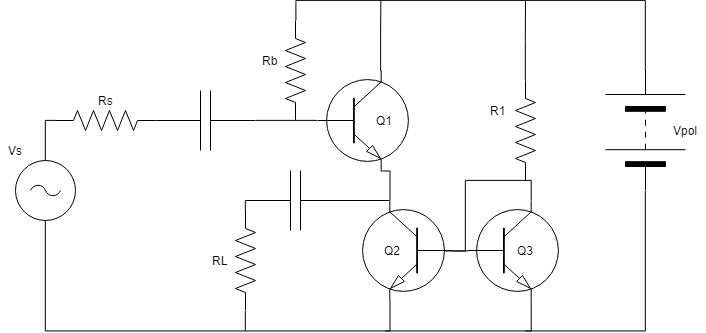
\includegraphics[scale=0.5]{imagenes/circuito.png}
	\caption{Amplificador}\label{fig:cir}
\end{figure}

Los valores de los componenetes del circuito son los indicados en la siguiente tabla:
\begin{table}[h]
\begin{center}
\begin{tabular}{|c|c|}
\hline
Componente& Valor\\
\hline \hline
$R_S$ & $560 \Omega$  \\ \hline
$R_L$ & $2.2 K \Omega$  \\ \hline
$R_B$ & $680 K \Omega$  \\ \hline
$R_1$ & $10K\Omega$  \\ \hline
$C$ & $1uF$  \\ \hline
$V_{POL}$ & $20V$  \\ \hline
$Q_1 = Q_2 = Q_3$ & BC547  \\ \hline

\end{tabular}
\caption{Tabla de componentes} \label{tab:comp}
\end{center}
\end{table}


Las caracterisiticas de los transistores son las siguientes \footnote{Datasheet del BC547: Sparkfun.com. (2018). [online] Disponible en: https://www.sparkfun.com/datasheets/Components/BC546.pdf [Accedido 10 Nov. 2018].} :

\begin{table}[h]
\begin{center}
\begin{tabular}{|c|c|c|}
\hline
$H_{FE}$(DC)& $h_{fe}$ (AC)&$V_A$\\
\hline \hline
110&165 &$98\mathrm{V}$\\ \hline

\end{tabular}
\caption{Caracter\'isiticas de los transistores} \label{tab:qcar}
\end{center}
\end{table}

\subsection{Análisis del amplificador}
En esta sección se analizar\'a la polarización y las características de pequeñas señales del amplificador.
\subsubsection{Polarización}
Para analizar la polarización del circuito, se pasivar\'an las fuentes del alterna. Lo primero a calcular es la fuente de corriente de la figura \ref{fig:ms}.

\begin{figure}[H]	
	\centering
	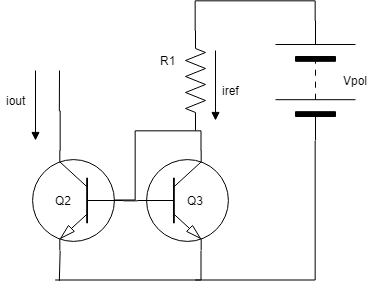
\includegraphics[width=0.4\textwidth]{imagenes/mirrorsource.png}
	\caption{Fuente de corriente constante}\label{fig:ms}
\end{figure}
Suponiendo que $Q_2$ y $Q_3$ son transistores iguales, tambien sus corrientes de base son iguales, y por ende sus corriente de colector también lo son, y asumiendo que la corriente de base es despreciable frente a la de colector, entonces $I_{OUT}=I_{REF}$. 
\par Recorriendo la malla de entrada de $Q_3$ obtenemos que:
\begin{equation}
I_{REF}=\frac{V_{POL}-V_{BE}}{R_1}\label{eq:mss}
\end{equation}

Conociendo las características de la fuente de corriente, se analizara la polarización del circuito:

\begin{figure}[H]	
	\centering
	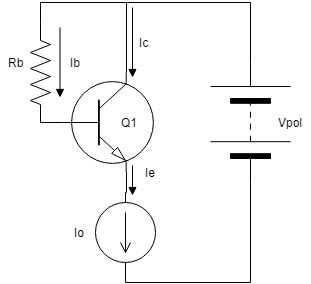
\includegraphics[width=0.4\textwidth]{imagenes/pol.png}
	\caption{Polarizaci\'on del amplificador}
\end{figure}

Como $I_E=I_O $, e $ I_O $ se obtiene a partir de la ecuación \ref{eq:mss}, entonces:
\begin{equation}
I_E=\left( H_{FE} +1 \right)  I_B=I_O
\end{equation}
despejando $I_B$ se obtiene:
\begin{equation}
I_B=\frac{I_O}{H_{FE}+1}
\end{equation}
\begin{equation}
I_{C}\cong I_O
\end{equation}

La tensión colector emisor se puede calcular de la siguiente manera:
\begin{equation}
V_C=V_{POL}
\end{equation}
\begin{equation}
V_E=V_{POL} - R_B I_B - V_{BE}
\end{equation}

Restando ambas expresiones obtenemos:

\begin{equation}
V_{CE}=I_B R_B + V_{CE}
\end{equation}

Finalmnete reemplazando con los valores de los componentes de las tablas \ref{tab:comp} y \ref{tab:qcar}, obtenemos :
$$I_B=17.5\mu \mathrm{A} $$
$$I_C=1.93 \mathrm{mA} $$
$$V_{CE}=12.6\mathrm{V} $$

\subsubsection{Modelo incremental}
Los tres transistores comparten la misma corriente de colector y también de base, ya que los tres transistores son iguales. Por ende poseen los  mismos parámetros híbridos.
$$\widehat{\frac{1}{h_{oe}}}\cong \frac{V_A}{I_{Cq}} $$
$$ \widehat{h_{ie}}\cong (h_{fe}+1)\frac{V_T}{I_{Cq}}$$

Evaluando las expresiones anteriores con los resultados obtenidos  anteriormente, y con el contenido de las tablas \ref{tab:comp} y \ref{tab:qcar}, obtenemos :

$$\frac{1}{h_{oe}}\cong 50.8\mathrm{k}\Omega $$
$$ h_{ie}\cong 2.2\mathrm{k}\Omega $$

\subsubsection{Circuito incremental}
En la siguiente figura se puede observar el circuito incremental del amplificador. $R_{OS}\cong \frac{1}{h_{oe}}\cong 50.8\mathrm{k}\Omega  $ es la impedancia de salida de la fuente espejo. 
\begin{figure}[H]	
	\centering
	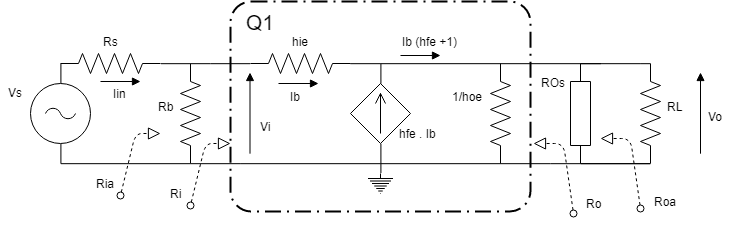
\includegraphics[width=0.9\textwidth]{imagenes/incr.png}
	\caption{Circuito incremental}
\end{figure}

A partir del circuito incremental se obtuvieron las siguientes relaciones:

\begin{equation}
R_D=\left( R_{L} // \frac{1}{h_{oe}} // R_{OS} \right)
\end{equation}
\begin{equation}
v_{O}=\left( h_{fe} +1 \right) i_{B} R_D
\end{equation}
\begin{equation}
v_{I}=\left( h_{fe} +1 \right) i_{B} R_D + h_{ie} i_{B} \label{eq:ri}
\end{equation}



Defieniendo $\Delta v =\frac{v_O}{v_I}$ y simplificando:

\begin{equation}
\Delta v =\frac{v_O}{v_I}=\frac{\left( h_{fe} +1 \right) R_D}{\left( h_{fe} +1 \right) R_D + h_{ie} }
\end{equation}

Tambien se define  $\Delta v_S =\frac{v_O}{v_S}$

\begin{equation}
\Delta v_S =\frac{v_O}{v_S}=\frac{v_I}{v_S} \frac{v_O}{v_I} =\frac{v_I}{v_S}\Delta V 
\end{equation}

Donde
\begin{equation}
\frac{v_I}{v_S} = \frac{R_{IA}}{R_{IA}+R_S}
\end{equation}

Dividiendo la ecuación \ref{eq:ri} por $i_B$ obtenemos $R_I$

\begin{equation}
R_I=\frac{v_I}{i_B} = \left( h_{fe} +1 \right) R_D + h_{ie}
\end{equation}

\begin{equation}
R_{IA}= R_I // R_B=\frac{R_I R_B}{R_I + R_B}
\end{equation}

Para hallar la impedancia de salida se pasiv\'o la fuente $v_S$, se conectó a la salida un generador y se calculó el cociente entre la tensión y la corriente.

\begin{equation}
R_O=\left( \frac{h_{ie} + \left( R_S // R_B \right)}{h_{fe}+1} \right) // \frac{1}{h_{oe}}
\end{equation}

\begin{equation}
R_{OA}=R_O // R_{OS}
\end{equation}

En cuanto a la ganancia de corriente $\Delta i=\frac{i_{R_L}}{i_{IN}}$:

\begin{equation}
\Delta i=\frac{R_B}{R_B +R_I} \frac{\left(  \frac{1}{h_{oe}} // R_{OS} \right)}{\left(  \frac{1}{h_{oe}} // R_{OS} \right) + R_L} (h_{fe} +1)
\end{equation}

Finalemente reemplazando por los valores obtenidos de las tablas \ref{tab:comp} y \ref{tab:qcar}, en las ecuaciones, se obtuvieron los siguientes valores:

$$\Delta v = 0.994$$
$$ \Delta v_S =0.991 $$
$$ R_I=338\mathrm{k}\Omega $$
$$ R_{IA} = 226\mathrm{k}\Omega $$
$$ R_O=13.3 \Omega $$
$$R_{OA}=13.3\Omega $$
$$\Delta i= 102 $$

\subsection{Medición del amplificador}
Se realizó el amplificador en protoboard (figura \ref{fig:pro}) y se midieron los parametros calculados anteriormente:

\begin{figure}[H]	
	\centering
	\fbox{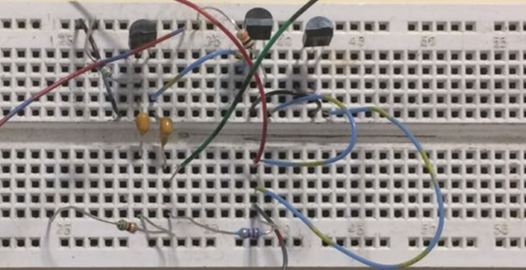
\includegraphics[width=0.5\textwidth]{imagenes/proto.png}}
	\caption{Circuito implementado}\label{fig:pro}
\end{figure}

$$\Delta v = 0.99$$
$$ \Delta v_S =0.99 $$
$$ R_{IA} = 175\mathrm{k}\Omega $$
$$R_{OA}=900\Omega $$
$$\Delta i= 78 $$


\section{Conclusión}
Comparando los resultados de la medición se observa que hay gran diferencia en las impedancias de entrada y de salida comparando con las te\'oricas. Esto se pudo deber a que el $h_{fe}$ utilizado no sea el correcto, debido a que el fabricante lo da en un rango, y los cálculos se realizaron con el t\'ipico. 
\par Las características más sobresalientes del circuito son su alta impedancia de entrada, su baja impedancia de salida, la ganancia de tensión es prácticamente uno y su alta ganancia de corriente.




\end{document}


